\chapter{Preprocessing image}
\section{Problem}
The propriety of an algorithm or a program often based on a good input set. To obtain the good result when applying the automatic classification methods. In this chapter, we suggest the algorithm preprocessing image. With the input images contains the parts of insect and an unexpected object, specifically yellow grid (figure \ref{fig:figure_31}), we need remove the yellow grid to have only insect and just keep the insect.
\begin{figure}[h!]
\centering
\subfloat[The yellow gird on the left of insect]{\label{fig:example_1}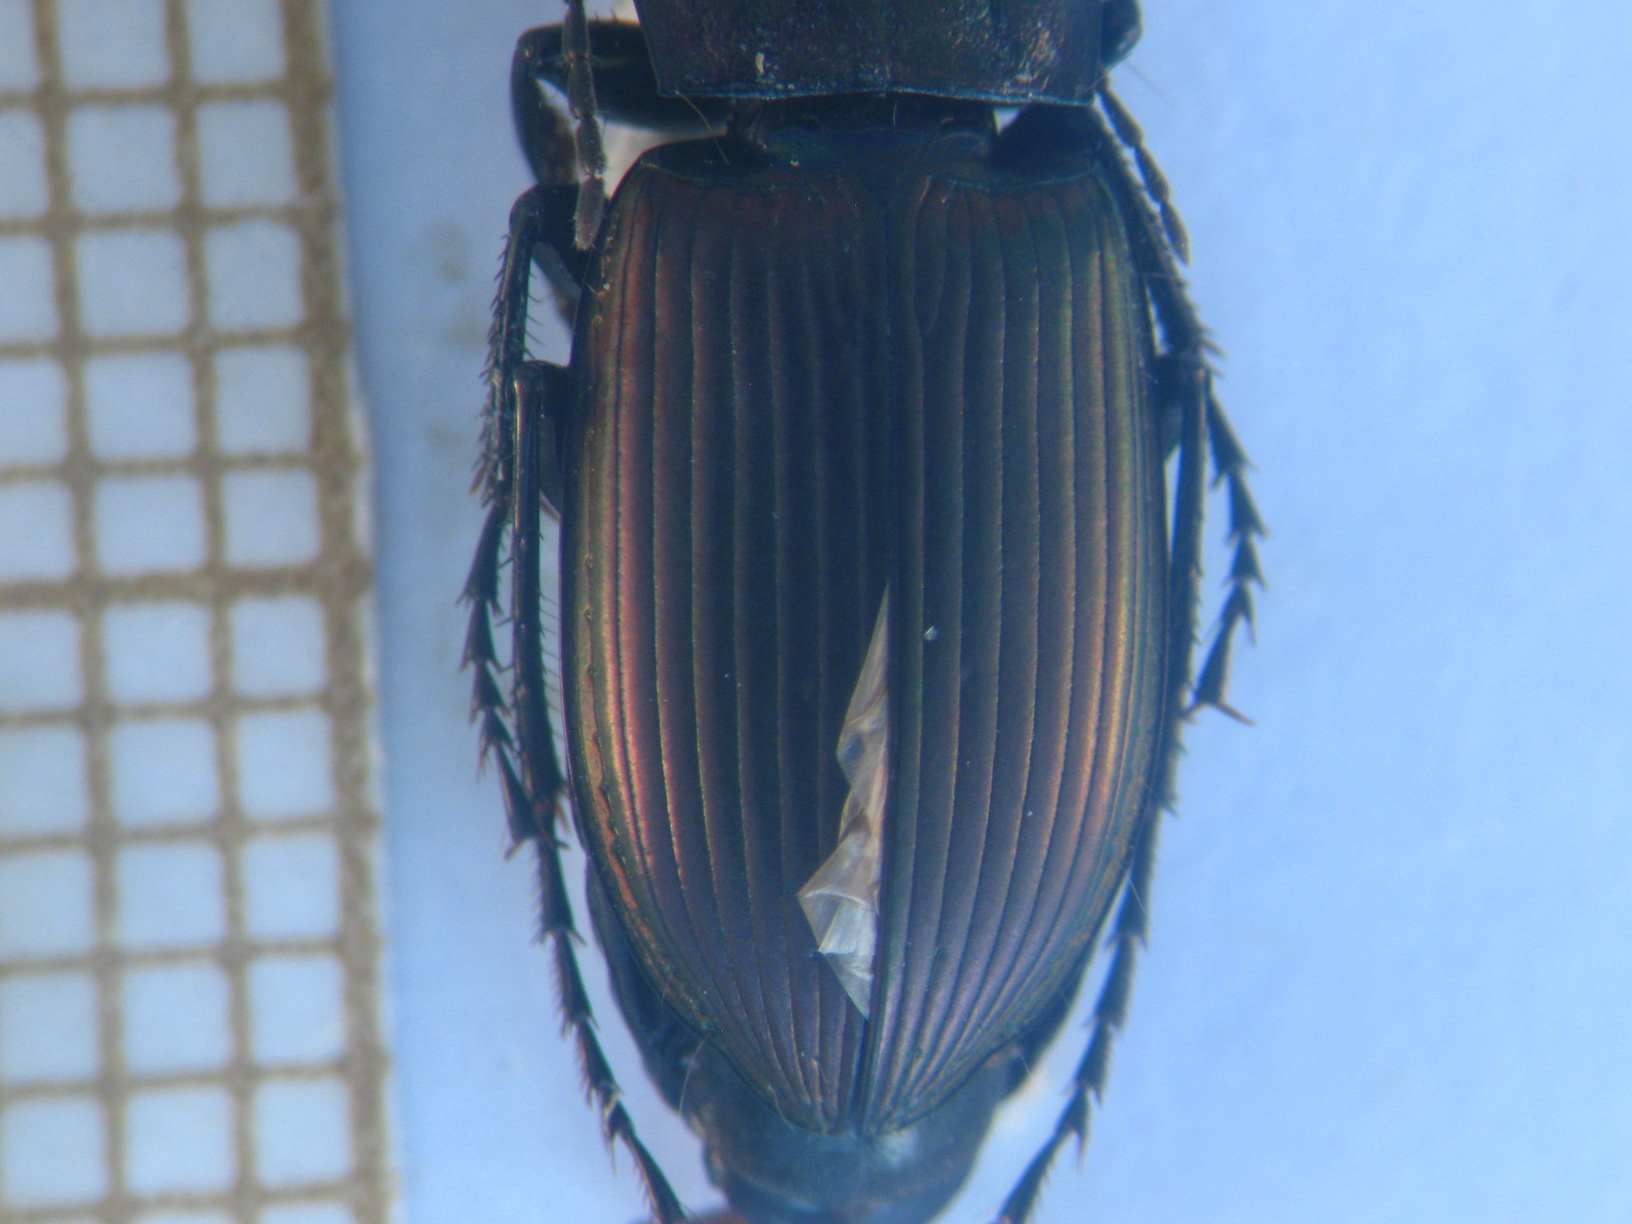
\includegraphics[width=0.4\textwidth]{./images/input1}}~~
\subfloat[The insect overlap the yellow grid]{\label{fig:example_2}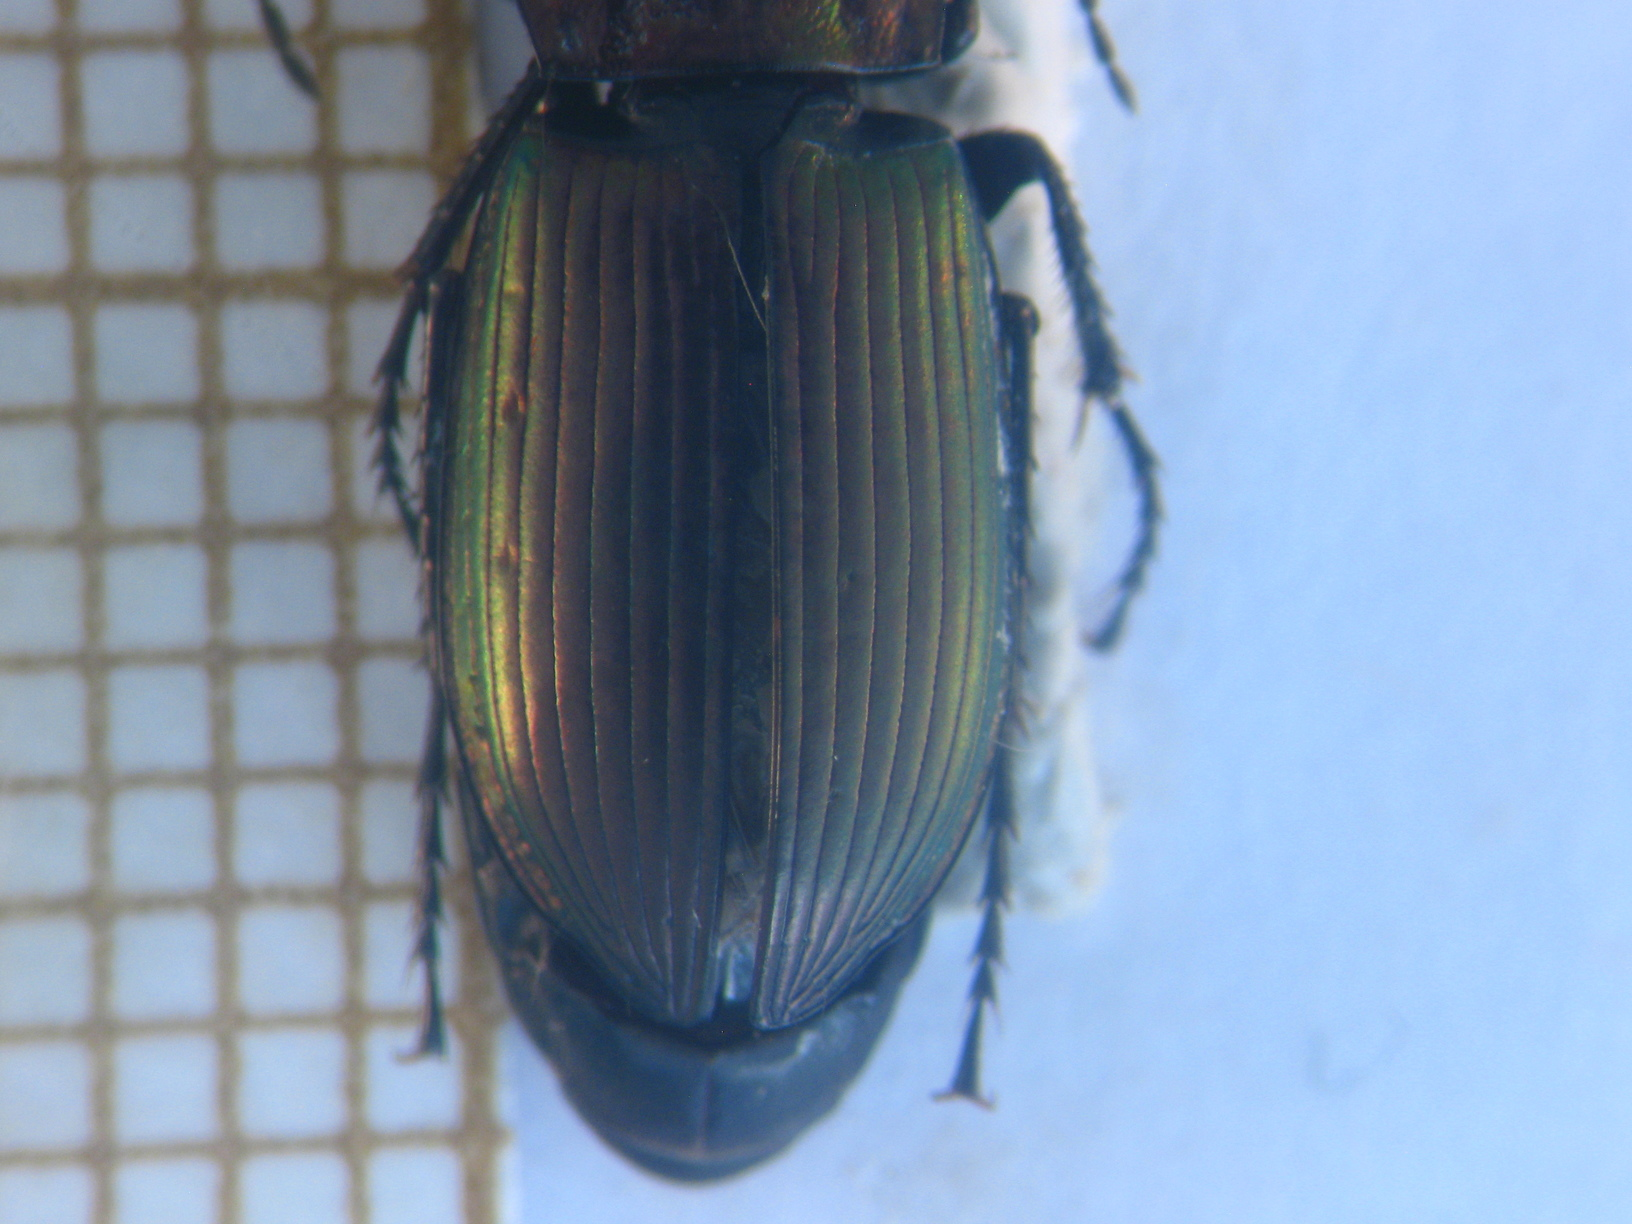
\includegraphics[width=0.4\textwidth]{./images/input2}}
\caption{The input images with yellow grid}
\label{fig:figure_31}
\end{figure}
\section{Analysis}
Each input image contains the two objects: the part of insect and the yellow grid (called grid). Addition, the grid always stayed in the left of image, and the insect can either overlap the grid or not. About the color, we can see three main groups color: the background color, the yellow color of grid and the color of insect. The image is presented in BGR model. So, the color at each pixel must be combine among three values (blue, green, red). If we process the image in BGR model, the algorithm may be complex. While, the HSV model just has a channel to present the value of color and each color has a clear range. We can apply this property for detecting and removing the gird. So, in this stage, we suggest that we convert the image to HSV model where has a clear range for each color and try to remove the yellow grid.\\
The analysis system is constructed from two main stages: finding the limiting and replacing points, replacing the yellow point from the begin to the limit point.
\subsection{Finding the limiting and the replacing point}
Browsing all of pixels to checking its color and replacing it if the color of pixel is yellow, we must process on all image. If we do that, it will be waste time. To decreasing the browsing time, in this step we find the limit points. These are the points which located on the right of grid and gird closest.\\
Finding the limit points will solve the above problem. Instance of checking on all pixel, we just check the pixels stay on the left of limit points. As we know, the width of grid usually less than a two-thirds of width of image. So, to reduce the time to finding the limit point, we also check from the begin of image to two-thirds of image. The result of this step is the limit points, these used for limiting the length when we check the pixels on yellow grid.\\
\textbf{The algorithm to find the limit points are followed:}\\
\begin{algorithm}[H]
\Indm
\KwData{inputImage: The input image (contains the insect and grid)}
\KwResult{The coordinate of limit point}
\Indp
Declare the variables\;
Convert image from BGR to HSV\;
Split HSV image into several channel
Set up initial \textit{limit\_point} and assign with the left-top corner.\;
Declare a variable $yellow\_count$ to count the number yellow points on each columns when processing. An column become a limit line if the number of yellow points on this column less than a constant value.\;
\For{$j \leftarrow 10 $ \KwTo $inputImage.columns$}{
	\If{H value at $(5,j) > $ 100 \\
		\textbar \textbar (H  value at $(5,j) > 70$\\
				$\&\&$ H value at $(5,j) < 100$\\
				$\&\&$ S value at $(5,j) < 10 $\\
				$\&\&$ V value at $(5,j) > 175$ )
		}{
		$limit\_point.x \leftarrow j$\;
		$limit\_point.y \leftarrow 0$\;
		$yellow\_count \leftarrow 0 $\; 
		\For{$i \leftarrow 1 $ \KwTo $grayImage.rows * 2/3$}{
			\If{H value at $(i,j) <= 38 $}{
				$yellow\_count++$\;
				\If{$yellow\_count >= 8$}{
					$limit\_point.x \leftarrow 0$\;
					$limit\_point.y \leftarrow 0$\;		
					break\;	
				}		
			}
		}
		\If{$limit\_point.x != 0$}{
			break\;
		}
	}
}
\If{$limit\_point.x == 0$}{
	$limit\_point.x \leftarrow inputImage.columns/3 + 200$\;
	$limit\_point.y \leftarrow 0$\;	
}
\caption{Algorithm to find the limiting points}
\end{algorithm}
Now, we indicate which is the color used to replace the yellow points. Hence, we choose the points having the value nearest with the background color. The histogram is ideal for choosing the position to replace, but we also have some conditions to obtain a good value.\\
The algorithm to find the replacing points are 
followed:\\
\IncMargin{1em}
\begin{algorithm}[H]
\Indm 
\KwData{inputImage: the input image}
\KwResult{The coordinate of replacing point}
\Indp
Convert image to gray scale image\;
Calculate the histogram on gray scale image and mean of histogram\;
Find the limit point:\;
\For{$i \leftarrow 0 $ \KwTo $grayImage.rows$}{
		\For{$j \leftarrow 0 $ \KwTo $grayImage.columns$}{
		\If{value at $(i,j) > $mean of histogram\\
			$\&\&$ H value (i,j) $>$ 90\\
			$\&\&$ H value (i,j) $>$ 130\\
			$\&\&$ S value at (i,j) $>$ 50\\
			$\&\&$ V value at (i,j) $>$ 215 }{
			return this position \;
		}
	}
}

\caption{Algorithm to find the replacing point}
\end{algorithm}\DecMargin{1em}
\subsection{Replacing the grid}
After having the limit points. By processing on all rows of image. At each row, we replace the pixels which have the color value stay in the range of yellow by another value. But the grid is not only created by the yellow point, it contains more the pixel have the value stay in the same range with background. But the brightness of these pixels is less than the background. So, we needs to replace it obtained the good image. In each row, this work repeated until meeting the limit points or a ``special point" (called ``break" point). It can be a point stayed on the insect or a point belong to background.\\
For each part of the insect, the color on insect or the background also have the difference value. So, we establish the difference values for each part. Based on the file name of image, we can classify it.\\
\IncMargin{1em}
\begin{algorithm}[H]
\Indm
\KwData{filePath: the file path of image}
\KwResult{Which part of insect in image}
\Indp
\textit{QString} temp $\leftarrow$ filePath.toLower()\;
\If{temp contains ``ely"}{
	return ELYTRE\;
}
\If{temp contains ``md"}{
	return MDROITE\;
}
\If{temp contains ``mg"}{
	return MGAUCHE\;
}
\If{temp contains ``prono"}{
	return PRONOTUM\;
}
\If{temp contains ``tete"}{
	return TETE\;
}
return ELYTRE\;
\caption{Algorithm to get the parts of insect}
\end{algorithm}
\DecMargin{1em}
\IncMargin{1em}
\begin{algorithm}[H]
\Indm
\KwData{inputImage: the input image; limit\_point: the limit point; part: part of insect; minBrightness: minimum of brightness; rpoint: replacing point}
\KwResult{The image after replace the yellow grid}
\Indp
\For{$i \leftarrow 0 $ \KwTo $inputImage.rows$}{
		\For{$j \leftarrow 0 $ \KwTo $limit\_point.x$}{
		\If{part is ELYTRE}{
			\If{ value at $(i,j+50)$ satisfy breaking condition}{
				break\;
			}
		}
		\If{part is MDROITE or MGAUCHE}{
			\If{ value at $(i,j+50)$ satisfy breaking condition}{
				break\;
			}
		}
		\If{part is PRONOTUM}{
			\If{ value at $(i,j+50)$ satisfy breaking condition}{
				break\;
			}
		}
		\If{part is TETE}{
			\If{ value at $(i,j+50)$ satisfy breaking condition}{
				break\;
			}
		}
		\If{H value at $(i,j+50)$ in yellow range}{
			replace value at this point by the value at replacing point\;
		}\lElse{
			\If{V at $(i,j+50) > $ minBrightness}{
				replace value at this point by the value at replacing point\;
			}
		}
	}
}
Merging three channel of HSV\;
Convert the image from HSV to BGR\;
\caption{Algorithm to replace the yellow grid}
\end{algorithm}
\DecMargin{1em}
\section{Summary}
In this chapter, we propose a method to remove the grid in the image. In short, the algorithm have steps followed:\footnote{The algorithm is combined from the algorithms in each step, which was described above.}
\begin{enumerate}
\item Converting the input image to HSV model
\item Splitting the image (in HSV) to get the individual channel
\item Finding the limit points
\item Choosing the replace point (calculating the histogram and mean value)
\item Getting the type of input and establish the break conditions.
\item Finding and replacing the yellow points and the ``miss brightness" point.
\item Merging the channels of HSV
\item Converting the HSV image to BGR image
\end{enumerate}







































